\documentclass{article}

\usepackage[parfill]{parskip}
\usepackage{graphicx}

\overfullrule=2cm

\begin{document}

\title{TDDC17: Lab 2}
\author{Henning Hall \& Anton Niklasson}
\maketitle


\section*{Questions}

\section{In the vacuum cleaner domain in part 1, what were the states and actions? What is the branching factor?}

A state in that world concists of an x position and a y position.

The branching factor for each node ranged between 1 and 4.

\section{What is the difference between Breadth First Search and Uniform Cost Search in a domain where the cost of each action is 1?}

There is not difference between the two in that situation.

\section{Suppose that h1 and h2 are admissible heuristics (used in for example A*). Which of the following are also admissible?}
\textbf{a) (h1+h2)/2}

Admissable.

\textbf{b) 2h1}

Not admissable.

\textbf{c) max (h1,h2)}

Admissable.

\section{If one would use A* to search for a path to one specific square in the vacuum domain, what could the heuristic (h) be? The cost function (g)? Is it an admissible heuristic?}

The heuristic could be the block distance between the current node and the goal node.

The cost function could be something like the total amount of steps from the initial node.

\newpage

\section{Choose your three favorite search algorithms and apply them to any problem domain.\\Draw the search tree for them, also include the memory usage.}

We constructed a small graph that represents our way home from campus to Ryd. We look at each crossing as a node in the graph.
Below is a sketch of the graph including the cost to move between the nodes:

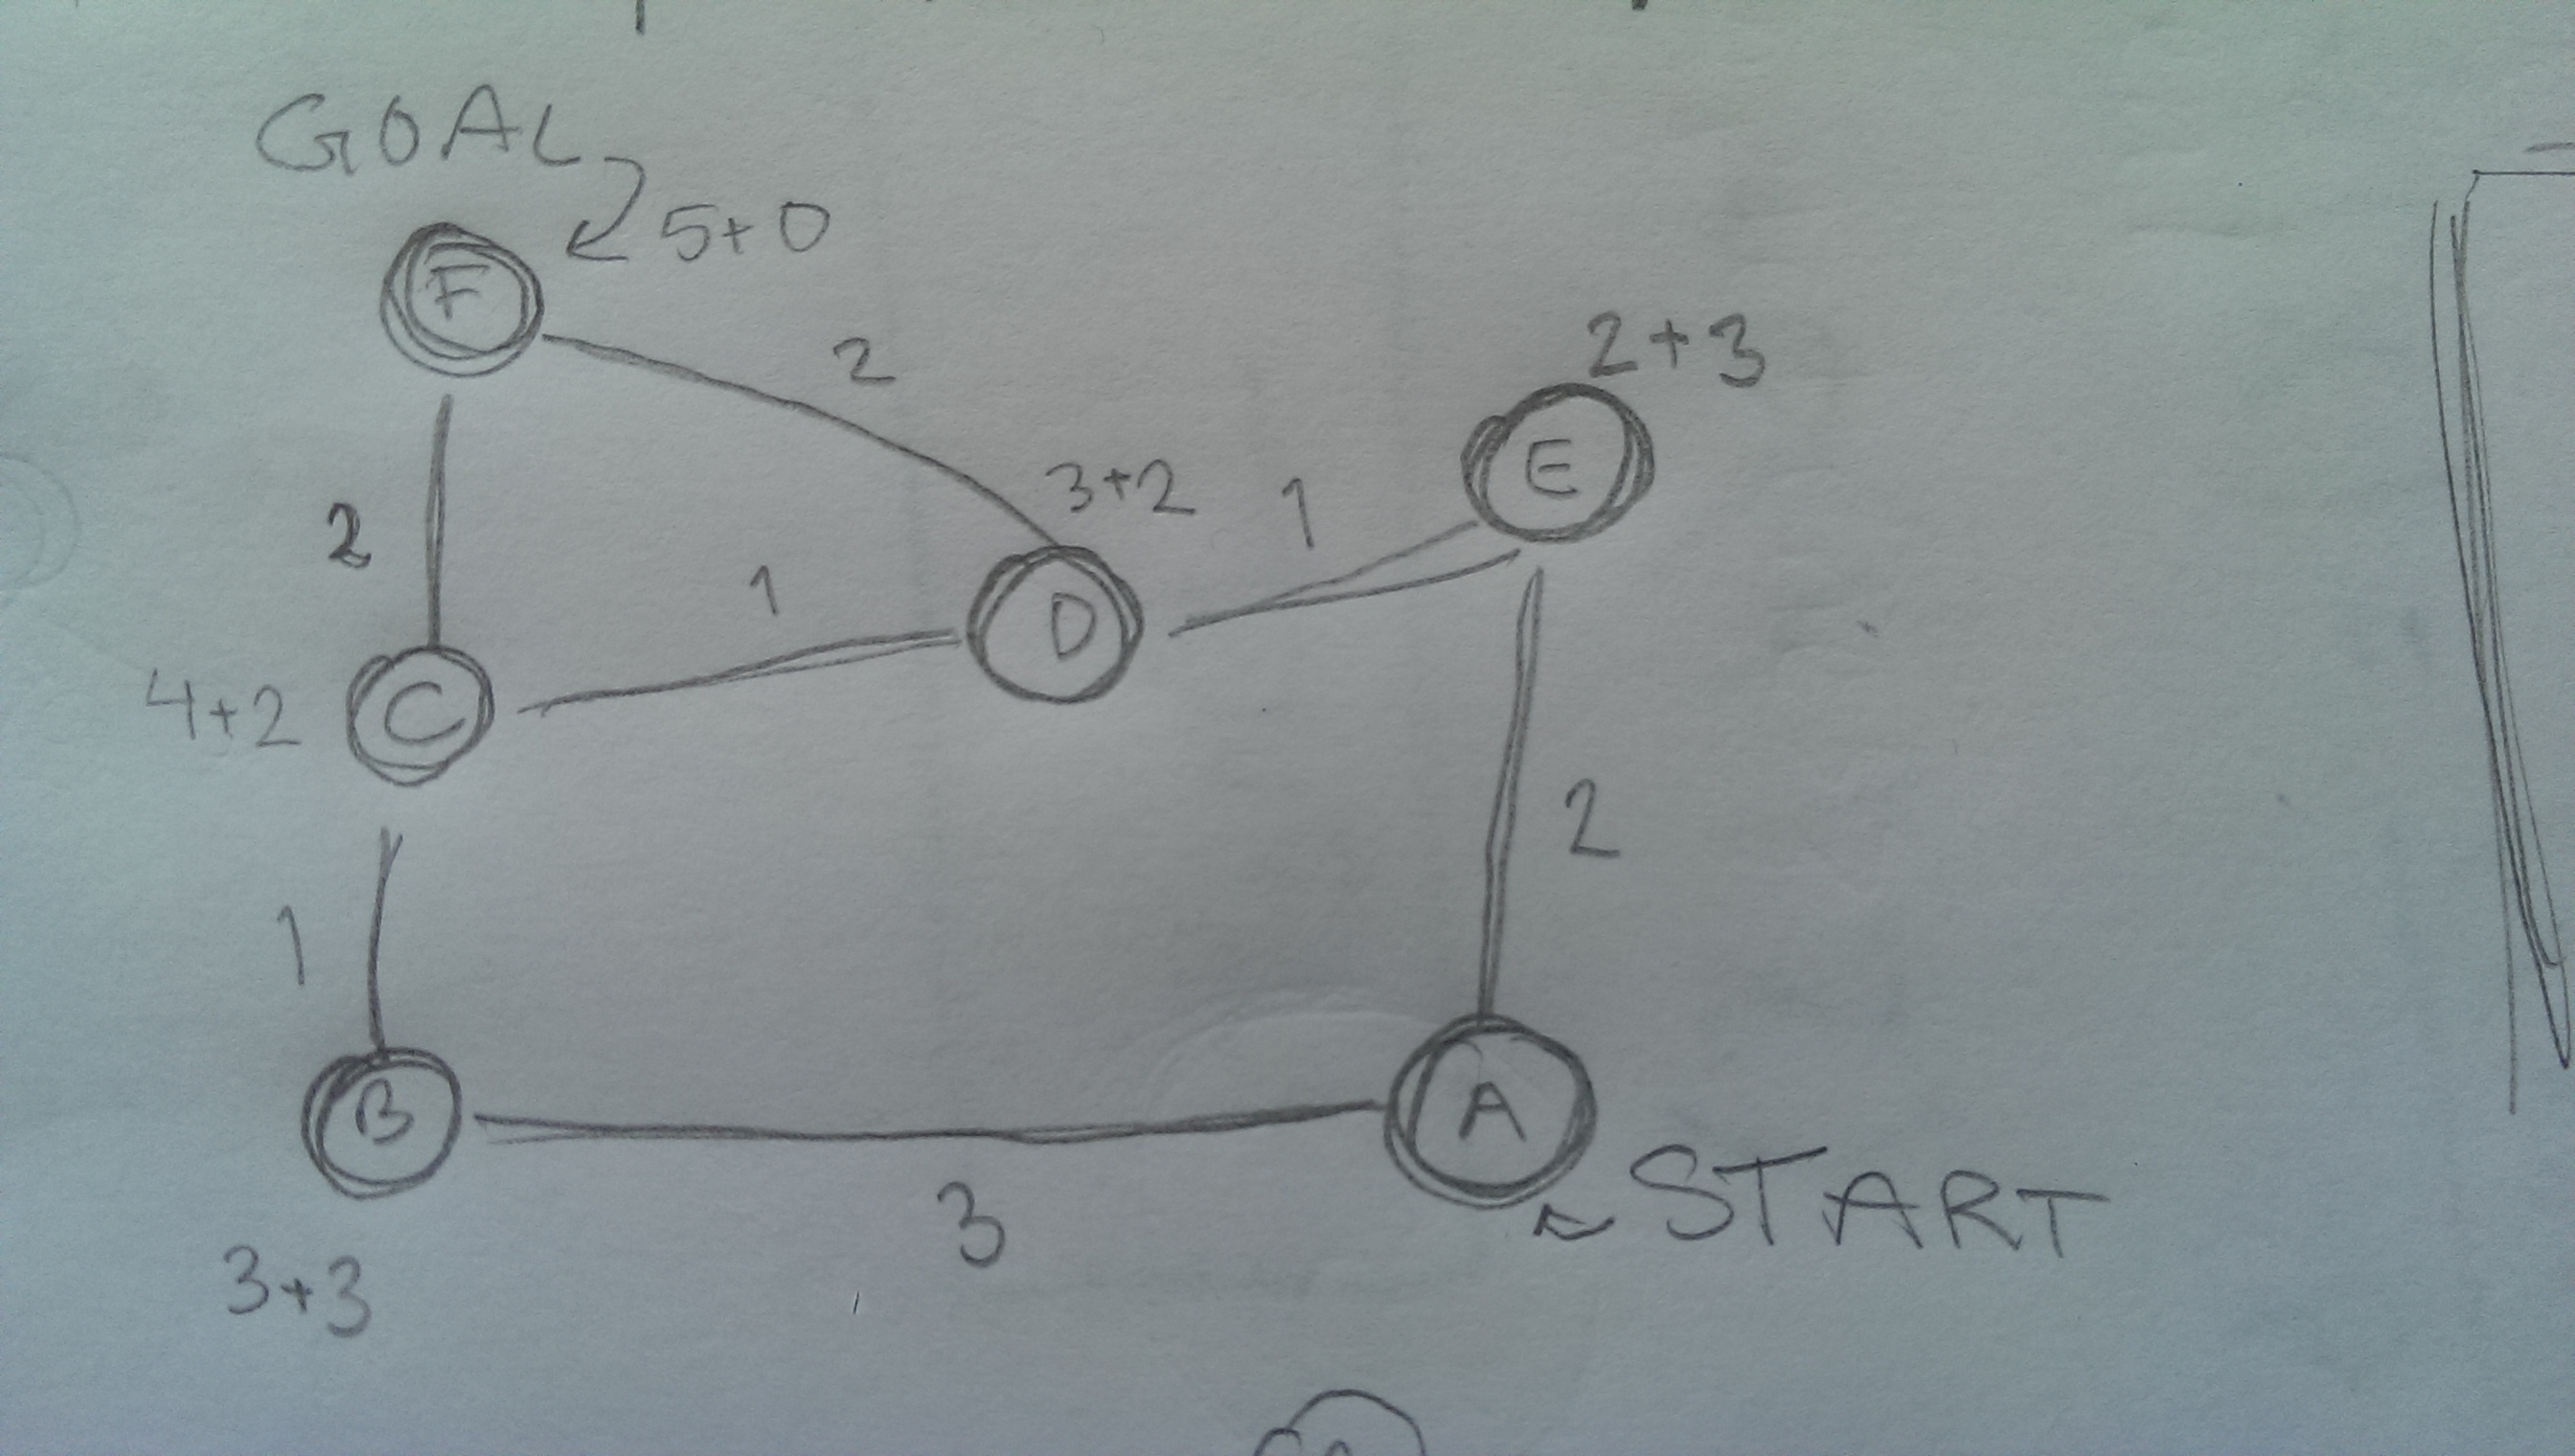
\includegraphics[scale=0.1]{graph}

We start our journey at Kårallen which we assigned the letter A. Our apartment is the node F. We chose to look at A*, DPS and BFS.

\subsubsection{A* Search}

The table below represents the bee line between all the nodes in graph. This table is utilized in our A star heuristic.

\begin{center}
	\begin{table}[h]
		\begin{tabular}{|l|l|l|l|l|l|l|}
			\hline
			   & A 		& B 	& C 	& D 	& E 	& F \\
			\hline
			A  & - 		& 3 	& 3.5	& 3 	& 2 	& 5 \\
			\hline
			B  & 3 		& - 	& 1 	& 1.5 	& 4 	& 3 \\
			\hline
			C  & 3.5	& 1 	& - 	& 1 	& 2 	& 2 \\
			\hline
			D  & 3 		& 1.5 	& 1 	& - 	& 1 	& 2 \\
			\hline
			E  & 2 		& 4 	& 2 	& 1 	& -	 	& 3 \\
			\hline
			F  & 5 		& 3 	& 2 	& 2 	& 3 	& - \\
			\hline
		\end{tabular}
	\end{table}
\end{center}

So, the heursitic \textit{h} is the distance to the goal, and the cost function \textit{g} is the total cost from the start.

Memory usage of the A* algortihm is pretty high. It grows exponentially with the problem which is not ideal.

The order of which A* expands the nodes in graph looks like this: A, E, D, F, C.

\section{Look at all the offline search algorithms presented in chapter 3 plus A* search. Are they complete? Are they optimal? Explain why!}

Answer.

\section{Assume that you had to go back and do lab 1 once more, but this time with obstacles. Remember that the agent did not have perfect knowledge of the environment but had to explore it incrementally. Could you still use the search algorithms you have learned to guide the agent's execution? What would you search for? Give an example.}

Answer.


\end{document}
